\documentclass[12pt]{article}

% This first part of the file is called the PREAMBLE. It includes
% customizations and command definitions. The preamble is everything
% between \documentclass and \begin{document}.

\usepackage[margin=1in]{geometry}  % set the margins to 1in on all sides
\usepackage{graphicx}              % to include figures
\usepackage{amsmath}               % great math stuff
\usepackage{amsfonts}              % for blackboard bold, etc
\usepackage{amsthm}                % better theorem environments
\usepackage{amssymb} 
\usepackage{mathptmx}
\usepackage{enumerate}
\usepackage{listings}
\usepackage{xcolor}
\usepackage{forest}
\usepackage{tabularx}  

% various theorems, numbered by section

\newtheorem{thm}{Theorem}[section]
\newtheorem{lem}[thm]{Lemma}
\newtheorem{prop}[thm]{Proposition}
\newtheorem{cor}[thm]{Corollary}
\newtheorem{conj}[thm]{Conjecture}
\newtheorem{mydef}[thm]{Definition}
\lstset{
	basicstyle          =   \sffamily,          
	keywordstyle        =   \bfseries,          
	commentstyle        =   \rmfamily\itshape,  
	stringstyle         =   \ttfamily,  
	flexiblecolumns,                
	numbers             =   left,   
	showspaces          =   false,  
	numberstyle         =   \fontsize{5}{skip},    
	showstringspaces    =   false,
	captionpos          =   t,      
	frame               =   lrtb,   
}

\lstdefinestyle{cpp}{
	language        =   cpp, 
	basicstyle      =   \fontsize{5}{skip},
	numberstyle     =   \fontsize{5}{skip},
	keywordstyle    =   \color{blue},
	keywordstyle    =   [2] \color{teal},
	stringstyle     =   \color{magenta},
	commentstyle    =   \color{red}\ttfamily,
	breaklines      =   true,   
	columns         =   fixed,  
	basewidth       =   0.5em,
}
\begin{document}


\title{ CSE 102 Spring 2021\\
	Quiz Reflection 6}

\author{Jaden Liu \\ 
University of California at Santa Cruz\\
Santa Cruz, CA 95064 USA }

\maketitle


\section{Quiz 6}
\begin{proof}[Solution for 1]
	c): Since the station is not divisible, we don't need exponential number to represent it. Thus, it's false\\
	d): 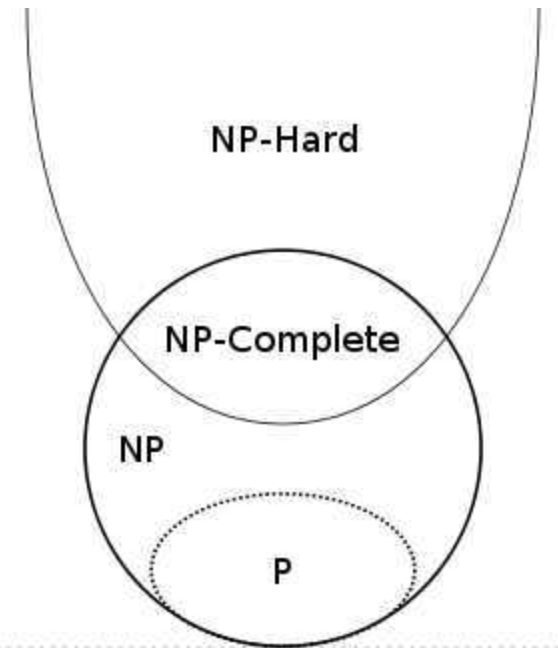
\includegraphics[scale=0.25]{1.png}
\end{proof}
\begin{proof}[Solution for 2]
	I misunderstand the meaning of the connected graph. So, we need to use the adversary strategy, answer no until it will generate a not connected graph.\\
	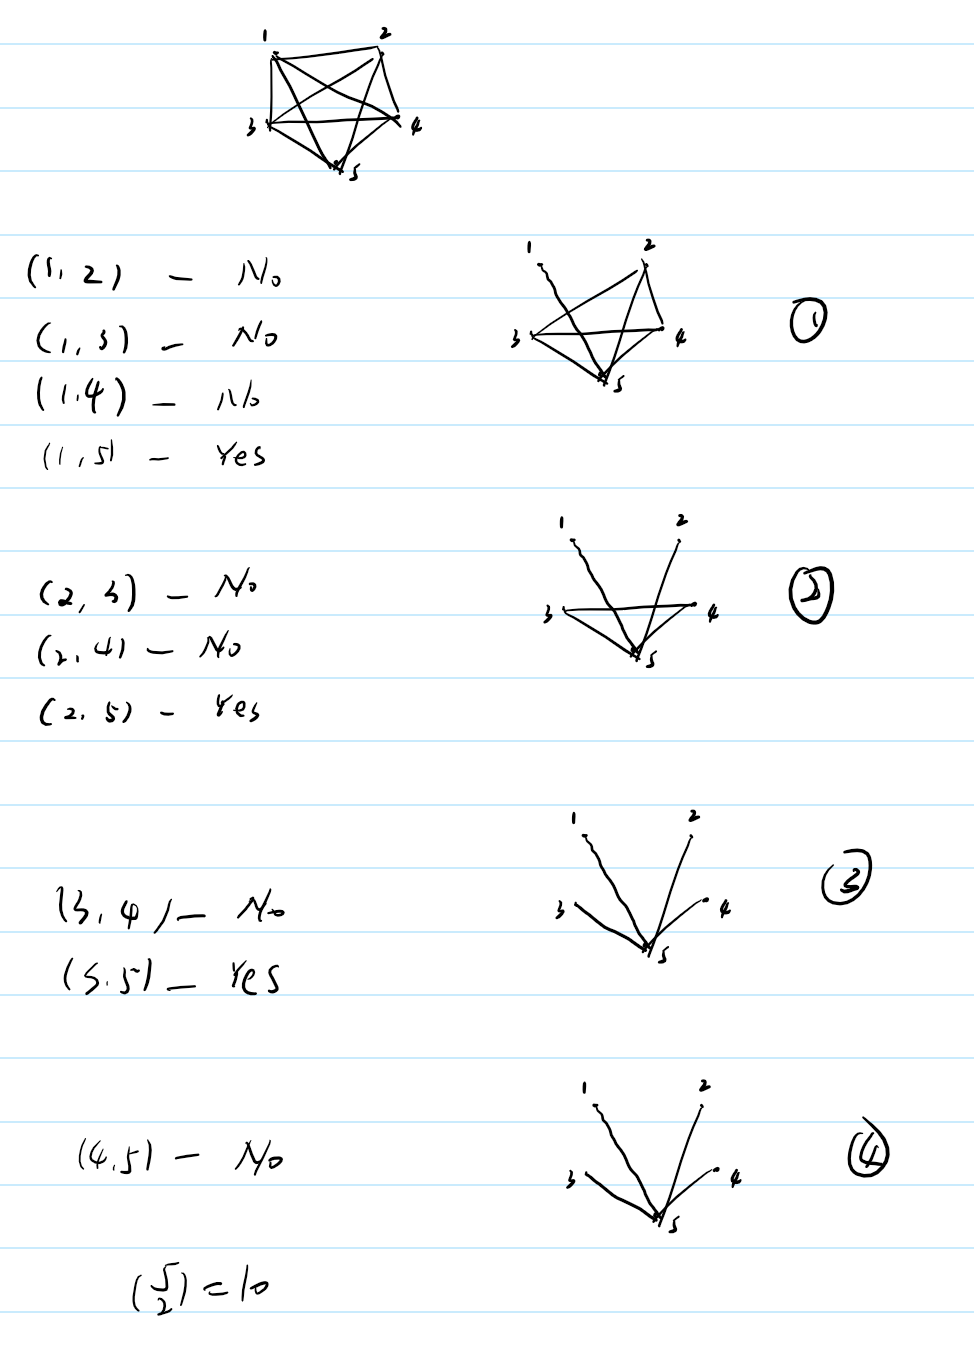
\includegraphics[scale=0.26]{2.png}
\end{proof}
\begin{proof}[Solution for 4]
	We need to first peek x2(or x3). Then we need peek at most 3 times.\\
	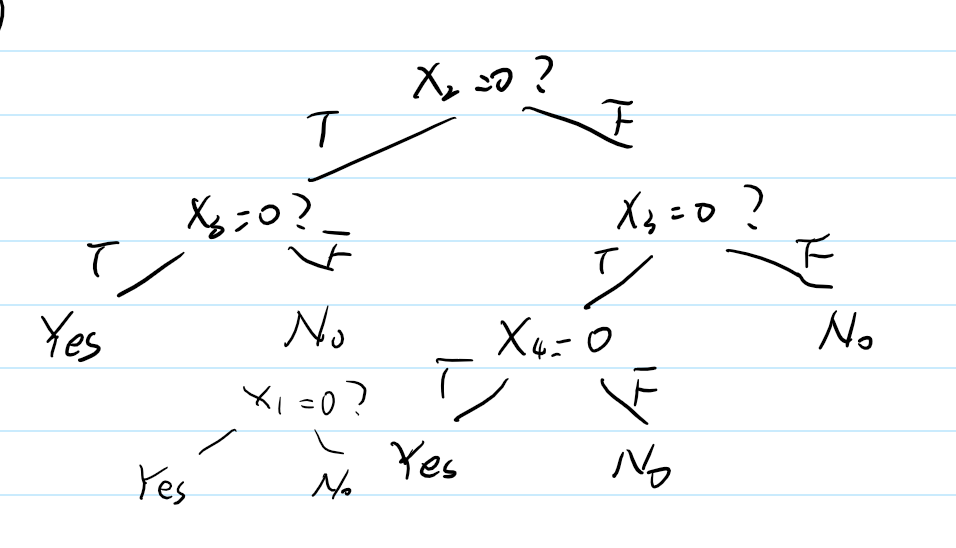
\includegraphics[scale=0.25]{4.png}
\end{proof}
\begin{proof}[Solution for 5]
	Since it's real-valued function, we have infinite possibilities.\\
	Assume we have a function $f(x)=256\cdot\frac{1}{x}$, this function satisfy the property that f(x) is monotonnically decreasing, f(1)=256. The stategy is just answer not negative to the gusser then generating the above result which is never negative.
\end{proof}



\bigskip



\end{document}
